\chapter{Despliegue del sistema}\label{cap:despliegue}
Una vez desarrollado el sistema, es necesario desplegarlo en un servidor para que los usuarios de la UGR puedan hacer uso de él. Para ello, se ha optado por contenerizar el sistema utilizando Docker, lo que permite una fácil gestión y escalabilidad de los microservicios que componen la aplicación.
\newline\newline
\textbf{**Revisar este párrafo y detallar más si necesario}
El servidor en el que se despliega el sistema se encuentra en el edificio auxiliar de la ETSIIT. Fue solicitado por el director del TFG, Juan Luis Jiménez Laredo, y facilitado por el CSIRC (Servicio de Ciberseguridad y Respuesta a Incidentess Informáticos) de la UGR. El servidor cuenta con las siguientes características:

Además se solicitó una IP estática para el servidor, que se ha configurado para que apunte al dominio \texttt{tempus.ugr.es}. 
Esto se ha conseguido gracias a la colaboración del CSIRC, que ha configurado el DNS para que apunte al servidor y al dominio.

\section{Configuración del servidor}
Como paso previo a la contenerización del sistema y despliegue de la aplicación, se ha procedido a la configuración del servidor. 
\newline\newline
Esta configuración fue realizada tanto por el director como por el autor del TFG:
\begin{itemize}
    \item Creación de usuarios y grupos necesarios para el despliegue de la aplicación.
    \item Instalación de Docker y Docker Compose. Configuración de Docker para que se ejecute como servicio al iniciar el sistema.
    \item Configurar ssh para permitir el acceso remoto al servidor, y scp para la transferencia de archivos.
    \item Instalar git para poder clonar los repositorios necesarios.
\end{itemize}

No hubo más pasos previos a la contenerización del sistema, y en gran parte esta es la ventaja de contenerizar el sistema, ya que permite una fácil gestión y despliegue de la aplicación sin necesidad de realizar configuraciones complejas en el servidor.
\newline\newline
Sin hacer uso de esta tecnología se habrían tenido que realizar, entre otros, los siguientes pasos:
\begin{itemize}
    \item Configuración de un servidor web (Apache) para servir la aplicación.
    \item Configuración de un servidor de base de datos (MySQL y MongoDB) para almacenar los datos de la aplicación.
    \item Instalación y configuración de Java y Maven para compilar y ejecutar los microservicios.
    \item Instalación y configuración de Node.js y Angular CLI para compilar el frontend de la aplicación.
    \item Configuración de un servidor de mensajería (RabbitMQ) para la comunicación entre microservicios.
    \item etc
\end{itemize}

Para acceder al servidor de manera remota se ha utilizado la VPN de la UGR, que permite conectarse al servidor de forma segura y acceder a los recursos de la red de la universidad.
\newline
Y para el paso de archivos entre el servidor y el equipo local se ha utilizado el protocolo SCP (Secure Copy Protocol), que permite transferir archivos de forma segura a través de SSH.
\section{Contenerización del sistema}

El primer paso realizado en este sentido ha sido la contenerización del backend del sistema, que está compuesto por varios microservicios. 

\subsection{Pasos para la contenerización del backend}

En esta primera fase se han contenerizado, construido y levantado los servicios de la siguiente manera:

\begin{enumerate}
    \item Crear una red en docker:
    \begin{lstlisting}[language=bash]
        docker network create calendarugr
    \end{lstlisting}
    \item Generar los .jar de los microservicios, sin pasar los tests para una construcción sin conflictos para los servicios que ya están contenerizados:
    \begin{lstlisting}[language=bash]
        ./mvnw clean package -DskipTests
    \end{lstlisting}
    \item Crear las imágenes de los microservicios (Ej imagen de Eureka service):
    \begin{lstlisting}[language=bash]
        FROM amazoncorretto:21-alpine-jdk
        WORKDIR /app
        EXPOSE 8761
        COPY ./target/eureka-service-0.0.1-SNAPSHOT.jar eureka-service.jar

        ENTRYPOINT ["java", "-jar", "eureka-service.jar"]
    \end{lstlisting}
    \item Construir la imagen de docker:
    \begin{lstlisting}[language=bash]
        docker build -t eureka-service .
    \end{lstlisting}
    \item Para levantar los contenedores uno a uno (Ej levantando el contenedor de Eureka):
    \begin{lstlisting}[language=bash]
        docker run -d --name eureka-service --network calendarugr -p 8761:8761 eureka-service
    \end{lstlisting}
    \item Bajar las imágenes oficiales de mysql:8.0.41 y mongo:6.0.4, además de las imágenes de RabbitMQ:
    \begin{lstlisting}[language=bash]
        docker pull mysql:8.0.41
        docker pull mongo:6.0.4
        docker pull rabbitmq:3-management
    \end{lstlisting}
    \item Para levantar contenedores con variables de entorno (Ej levantando el contenedor de Mysql):
    \item \begin{lstlisting}[language=bash]
        docker run -p 3307:3306 --network calendarugr \
            -e MYSQL_ROOT_PASSWORD=...\
            -e MYSQL_USER=... \
            -e MYSQL_PASSWORD=... \
            -v /home/juanmi/mysql-scripts/init.sql:/docker-entrypoint-initdb.d/init.sql \
            --name mysql \
            mysql:8.0.41
    \end{lstlisting}
    \item El init.sql es un script que se ejecuta al iniciar el contenedor de Mysql, y se utiliza para crear la base de datos y las tablas necesarias para el funcionamiento del sistema. El script se encuentra en la carpeta \texttt{mysql-scripts} del proyecto.
    \begin{lstlisting}[language=sql]
        CREATE DATABASE IF NOT EXISTS DB_USER_SERVICE;
        CREATE DATABASE IF NOT EXISTS DB_SCHEDULE_CONSUMER_SERVICE;

        GRANT ALL PRIVILEGES ON DB_USER_SERVICE.* TO 'calendarugr'@'%';
        GRANT ALL PRIVILEGES ON DB_SCHEDULE_CONSUMER_SERVICE.* TO 'calendarugr'@'%';
        FLUSH PRIVILEGES;
    \end{lstlisting}
    \item Para levantar el contenedor de Mongo:
    \begin{lstlisting}[language=bash]
        docker run -d --name mongodb \
            -p 27018:27017 \
            --network calendarugr \
            -e MONGO_INITDB_ROOT_USERNAME=... \
            -e MONGO_INITDB_ROOT_PASSWORD=... \
            mongo:6.0.4
    \end{lstlisting}
\end{enumerate}

De esta manera se levantan todos los servicios uno a uno y se pueden probar de forma individual y en conjunto. Sin embargo, para facilitar el despliegue y la gestión de los microservicios, se ha optado por utilizar Docker Compose.

\subsection{Docker Compose}
Docker Compose es una herramienta que permite definir y ejecutar aplicaciones Docker multi-contenedor. Con Docker Compose, se puede definir la configuración de todos los microservicios en un único archivo \texttt{docker-compose.yml}, lo que facilita su gestión y despliegue.
\newline\newline
Este enfoque nos permite centralizar la configuración de todos los microservicios en un único archivo, lo que facilita su gestión y despliegue, de manera que:
\begin{itemize}
    \item Cada microservicio se define como un servicio en el archivo \texttt{docker-compose.yml}.
    \item Se especifican las imágenes de cada microservicio, los puertos que se exponen, las redes a las que pertenecen y las variables de entorno necesarias.
    \item Se definen las dependencias entre los servicios, lo que permite que Docker Compose gestione el orden de inicio de los contenedores.
    \item Se pueden definir volúmenes para persistir los datos de los servicios, como en el caso de MySQL y MongoDB.
\end{itemize}

De esta manera lo único que haría falta en el servidor para levantar todo el backend sería un directorio contenedor del archivo \texttt{docker-compose.yml}. Al tener este archivo referencia a las imágenes oficiales de MySql, Mongo y RabbitMQ, además de las imágenes de los servicios subidos a Docker Hub, no es necesario tener las imágenes construidas en el servidor, ya que Docker Compose se encargará de descargarlas automáticamente al levantar los servicios.

Para levantar todos los servicios definidos en el archivo \texttt{docker-compose.yml}, se puede ejecutar el siguiente comando:
\begin{lstlisting}[language=bash]
    docker-compose up -d ( -d para que se levanten en segundo plano)
\end{lstlisting}

Además para facilitar aún se han creado automatizaciones para la construcción de las imágenes y el despliegue de los microservicios, de manera que se pueden ejecutar los siguientes comandos:
\begin{lstlisting}[language=bash]
    ./build_services.sh 
    ./upload_to_hub.sh
\end{lstlisting}

Estos scripts se encargan de construir las imágenes de los microservicios y subirlas al repositorio de Docker Hub, lo que permite que se puedan desplegar en cualquier servidor con Docker instalado.

\subsection{Pasos para la contenerización del frontend}

El frontend del sistema está desarrollado en Angular y se ha decidido contenerizarlo utilizando Apache como servidor web. A continuación se detallan los pasos realizados para la dockerización del frontend:

\begin{enumerate}
    \item Construir el proyecto Angular para producción:
    \begin{lstlisting}[language=bash]
        ng build --configuration production
    \end{lstlisting}
    Este comando generará una carpeta \texttt{dist} con los archivos necesarios para desplegar la aplicación. Estos serán trasladados a un directorio del servidor, por ejemplo, \texttt{built\_tempus}, y deberá estar disponible en el mismo directorio que el docker-compose.yml, los certificados, y un directorio ``apache'' con el archivo de configuración de Apache y el Dockerfile.
    \newline
    Además, dentro del directorio \texttt{built\_tempus} se debe crear un archivo \texttt{.htaccess} con el objetivo de redirigir todas las peticiones al archivo \texttt{index.html} del frontend, para que Angular pueda manejar el enrutamiento de la aplicación. El contenido del archivo \texttt{.htaccess} es el siguiente:
    \begin{lstlisting}[language=bash]
        RewriteEngine On
        RewriteBase /
        RewriteRule ^index\.html$ - [L]
        RewriteCond %{REQUEST_FILENAME} !-f
        RewriteCond %{REQUEST_FILENAME} !-d
        RewriteRule . /index.html [L]
    \end{lstlisting}
    \item Solicitar los certificados SSL necesarios para el dominio \texttt{tempus.ugr.es}. Estos certificados son necesarios para habilitar HTTPS en el servidor web, y habilitarlo tanto para el frontend como para el backend.
    \item Copiar los certificados SSL en una carpeta del servidor, por ejemplo, en \texttt{/home/user/certificates}. Estos certificados son necesarios para habilitar HTTPS en el servidor web.
    \item Crear un archivo de configuración para Apache (\texttt{apache-ssl.conf}) en el que se especifique la configuración del servidor web.
          Aquí se especifican el uso de SSL, la redirección de HTTP a HTTPS y la configuración del \hyperlink{reverseproxy}{Reverse Proxy} para el backend.
        \begin{lstlisting}[language=bash] 
            <VirtualHost *:443>
                ServerName tempus.ugr.es
                ServerAlias xxx.xx.xxx.xxx

                # Directorio raiz donde se encuentra tu aplicacion Angular
                DocumentRoot /var/www/html

                # Habilitar SSL
                SSLEngine on
                SSLCertificateFile /ejemplo/de/ruta/certificado.pem                
                SSLCertificateKeyFile /ejemplo/de/ruta/clave-privada.pem

                # Configuracion de cifrados seguros
                SSLCipherSuite "HIGH:MEDIUM:!MD5:!RC4:!3DES"
                SSLHonorCipherOrder on

                # Protocolos seguros
                SSLProtocol -all +TLSv1.2 +TLSv1.3

                SSLProxyEngine On
                SSLProxyProtocol -all +TLSv1.2
                SSLProxyCheckPeerCN off
                SSLProxyCheckPeerName off

                # PROXY PARA EL API GATEWAY
                ProxyPass /calendarugr/v1 http://api-gateway:8090/calendarugr/v1
                ProxyPassReverse /calendarugr/v1 http://api-gateway:8090/calendarugr/v1

                <Directory /var/www/html>
                        Options Indexes FollowSymLinks
                        AllowOverride All
                        Require all granted
                    </Directory>

                    ErrorLog ${APACHE_LOG_DIR}/mi-app-error.log
                    CustomLog ${APACHE_LOG_DIR}/mi-app-access.log combined
                </VirtualHost>
        \end{lstlisting}
        Este archivo de configuración define un VirtualHost para el dominio \texttt{tempus.ugr.es} en el puerto 443 (HTTPS).
        \newline 
        Gracias a esta configuración, Apache actuará como un proxy inverso para el backend, redirigiendo las peticiones al API Gateway que se ejecuta en el contenedor de Docker.
    \item Creación del Dockerfile para el frontend, que se encargará de construir la imagen del contenedor que servirá la aplicación Angular. Este archivo irá en el mismo directorio que el archivo \texttt{apache-ssl.conf}.
        \begin{lstlisting}[language=bash]
            # Base image
            FROM ubuntu:latest

            ENV DEBIAN_FRONTEND=noninteractive

            # Install apache2
            # Install dependencies
            RUN apt-get update && apt-get install -y \
                php \
                apache2 \
                libapache2-mod-php \
                curl \
                && rm -rf /var/lib/apt/lists/*
            RUN apt-get update && apt-get install -y zip unzip git
            RUN apt-get install -y iputils-ping && apt install -y iproute2

            # Activate apache2 modules and enable SSL and proxy
            RUN a2enmod rewrite ssl proxy proxy_http && mkdir /etc/apache2/ssl
            # copy ssl files
            COPY ./apache-ssl.conf /etc/apache2/sites-available/apache-ssl.conf

            # activate the site
            RUN a2ensite apache-ssl.conf

            EXPOSE 443
        \end{lstlisting}
    \item Diseñar el archivo \texttt{docker-compose.yml} para el frontend, que incluirá la configuración del contenedor de Apache y la redirección de las peticiones al API Gateway.
    En este archivo hacemos que el contenedor del frontend use la misma red que el resto de microservicios, y que se levante el contenedor de Apache con la configuración del archivo \texttt{apache-ssl.conf}.
    \newline
    Además se especifica el volumen donde se encuentran los certificados SSL, el directorio \texttt{built\_tempus} que contiene los archivos del frontend y el archivo de configuración de Apache.

\end{enumerate}

El directorio contenedor de lo necesario para desplegar el frontend debería contener algo parecido a lo siguiente:
\begin{lstlisting}[language=bash]
    - apache-docker/
        - apache/
            - apache-ssl.conf         # Configuracion de Apache con SSL
            - DockerfileApache        # Dockerfile para construir el contenedor
        - certificados/
            - ClavePrivada.pem        # Clave privada SSL
            - Certificado.pem         # Certificado SSL
        - docker-compose.yml          # Composicion de servicios Docker
        - built_tempuis               # Carpeta donde se colocan los archivos de la app Angular
\end{lstlisting}

\section{Levantar el sistema}
Una vez que se han configurado y contenerizado todos los microservicios, se puede levantar el sistema completo utilizando Docker Compose. Para ello se debe levantar primero el backend, que es el que crea también la red de Docker necesaria para el frontend, y luego el frontend.
\newline
Con esto se consigue que el sistema esté completamente desplegado y accesible a través del dominio \texttt{tempus.ugr.es}.

\subsection{Paso del HTTP a HTTPS en las llamadas al backend}
Si sólo se levantara el backend exponiendo el puerto 8090 para las peticiones al api gateway, las peticiones al backend se realizarían a través de HTTP. Sin embargo, para que el sistema funcione correctamente y se pueda acceder a él a través del dominio \texttt{tempus.ugr.es}, es necesario que las peticiones al backend se realicen a través de HTTPS.
Para ello, se ha configurado Apache como un proxy inverso que redirige las peticiones al backend a través de HTTPS. De esta manera, las peticiones al backend se realizan a través del dominio \texttt{tempus.ugr.es} y el puerto 443, que es el puerto por defecto para HTTPS.

Ejemplo de endpoint del backend al que se accede a través de HTTP:

\lstset{inputencoding=utf8}
\begin{lstlisting}[language=bash]
http://172.25.190.139:8090/calendarugr/v1/schedule-consumer/classes-from-group
\end{lstlisting}

Ejemplo de endpoint del backend al que se accede a través de HTTPS:

\lstset{inputencoding=utf8}
\begin{lstlisting}[language=bash]
https://tempus.ugr.es/calendarugr/v1/schedule-consumer/classes-from-group
\end{lstlisting}

\subsection{Pruebas de carga en un entorno real}

Una vez todo lo necesario levantado para un funcionamiento normal del sistema, se han realizado pruebas de carga en un entorno real para comprobar el rendimiento y la escalabilidad del sistema. Estas pruebas se han realizado utilizando Locust \cite{locust}, que es una herramienta de código abierto para realizar pruebas de carga y rendimiento en aplicaciones web.
\newline\newline
Las pruebas de carga se han realizado para distintos usuarios (con una media de diez suscripciones a grupos de asignatura) solicitando la información de su calendario entero (acción más común del sistema), al endpoint \texttt{https://tempus.ugr.es/calendarugr/v1/academic-subscription/entire-calendar}.\newline
Además las solicitudes no se han hecho directamente al backend mediante llamadas http, sino que se han hecho a través del dominio \texttt{tempus.ugr.es}, que es el que se utiliza para acceder al sistema desde el navegador. Esto permite simular un uso real del sistema, ya que los usuarios acceden al sistema a través del dominio y no directamente al backend.
\newline
Sabiendo que en la UGR hay aproximadamente 60.000 estudiantes, y que el número de profesores :
\begin{itemize}
    \item Pruebas de carga con 100 usuarios concurrentes, simulando un uso normal del sistema.
    \item Pruebas de carga con 500 usuarios concurrentes, simulando un uso intensivo del sistema.
    \item Pruebas de carga con 1000 usuarios concurrentes, simulando un uso extremo del sistema.
\end{itemize}

Los parámetros que mide la herramienta son los siguientes:
\begin{enumerate}
    \item \textbf{Req.}: Número total de solicitudes realizadas.
    \item \textbf{Fails}: Número de solicitudes que han fallado.
    \item \textbf{Med(ms)}: Tiempo medio de respuesta en milisegundos.
    \item \textbf{95\%ile (ms)}: Tiempo de respuesta en el percentil 95 ( es decir, el 95\% de las solicitudes se han respondido en este tiempo o menos).
    \item \textbf{99\%ile (ms)}: Tiempo de respuesta en el percentil 99 ( es decir, el 99\% de las solicitudes se han respondido en este tiempo o menos).
    \item \textbf{Avg(ms)}: Tiempo medio de respuesta en milisegundos.
    \item \textbf{Min(ms)}: Tiempo mínimo de respuesta en milisegundos.
    \item \textbf{Max(ms)}: Tiempo máximo de respuesta en milisegundos.
    \item \textbf{Avg size(bytes)}: Tamaño medio de la respuesta en bytes.
    \item \textbf{RPS}: Solicitudes por segundo.
    \item \textbf{Fails/s}: Fallos por segundo.
\end{enumerate}


\subsubsection{Pruebas de carga con 100 usuarios concurrentes}

En esta prueba se simularon 100 usuarios concurrentes realizando solicitudes al sistema durante 2 minutos. Los resultados obtenidos fueron los siguientes:

\begin{table}[H]
\centering
\resizebox{16cm}{!}{
\begin{tabular}{|r|r|r|r|r|r|r|r|r|r|r|}
\hline
\textbf{Req.} & \textbf{Fails} & \textbf{Med(ms)} & \textbf{95\%(ms)} & \textbf{99\%(ms)} & \textbf{Avg(ms)} & \textbf{Min(ms)} & \textbf{Max(ms)} & \textbf{Avg size(Bytes)} & \textbf{RPS} & \textbf{Fails/s} \\
\hline
4172 & 35 & 84 & 120 & 6300 & 213.04 & 1 & 7329 & 9636.47 & 32.2 & 0.1 \\
\hline
\end{tabular}
}
\caption{Resultados de la prueba de carga con 100 usuarios concurrentes.}
\label{tab:locust100}
\end{table}

\begin{figure}[H]
\centering
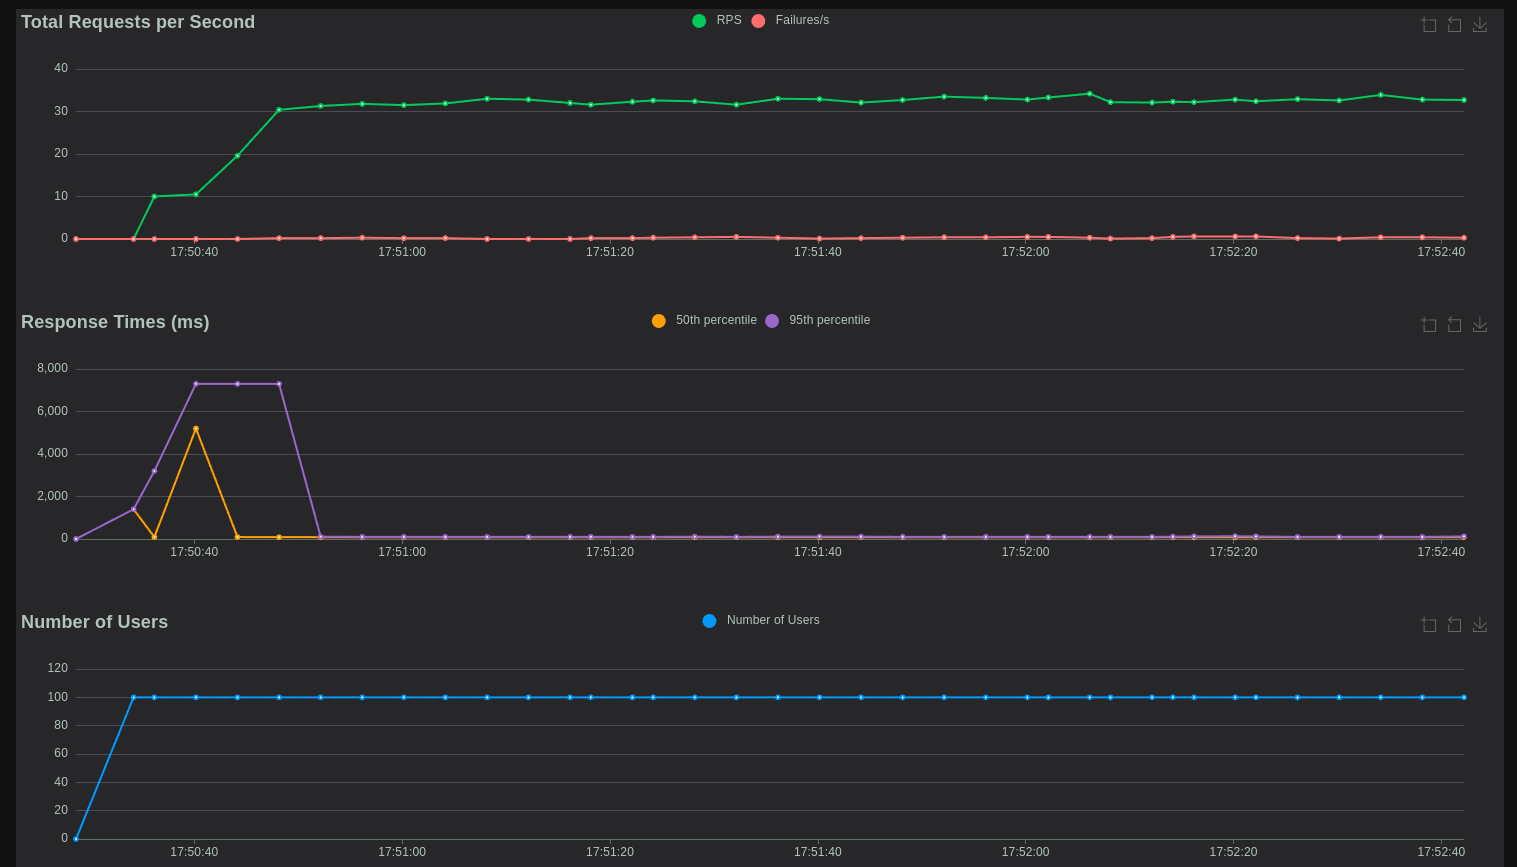
\includegraphics[width=0.9\textwidth]{figures/08_100_1.png}
\caption{Gráfica de la prueba de carga con 100 usuarios concurrentes.}
\label{fig:locust100}
\end{figure}

Se ha observado en la gráfica de ``Response Times (ms)'' un pico inicial de latencia significativa. Aproximadamente entre las 17:30:00 y 17:40:00, el percentil 95 alcanzó hasta 7300 ms (7 segundos) y el percentil 50 (mediana) llegó a unos 5200 ms (5 segundos). Posteriormente, los tiempos de respuesta se estabilizaron rápidamente, lo que es consistente con las estadísticas globales de la prueba, que muestran una mediana de 84 ms y un percentil 95 de 120 ms para el total de la ejecución.
\newline\newline
Este comportamiento es típico de un ``arranque en frío'' o ``cold start'' del sistema, que puede involucrar varios factores:

\begin{itemize}
    \item \textbf{Carga inicial de código:} Al inicio de la prueba, el servidor de aplicaciones necesita cargar el código en memoria, inicializar módulos, frameworks y establecer las primeras conexiones a la base de datos. Este proceso inicial consume tiempo.
    \item \textbf{Calentamiento de cachés:} Las aplicaciones web y las bases de datos (PostgreSQL) utilizan cachés. En las primeras solicitudes, estas cachés están vacías, y los datos deben ser recuperados de fuentes más lentas (disco o base de datos), lo que aumenta la latencia. Conforme más solicitudes llegan, las cachés se llenan, mejorando los tiempos de respuesta.
    \item \textbf{Pool de conexiones:} La creación y llenado del pool de conexiones a la base de datos es una operación relativamente costosa que ocurre al inicio.
    \item \textbf{Menor concurrencia inicial:} A pesar de un rápido incremento a 100 usuarios en la gráfica, las primeras solicitudes pueden impactar un sistema que aún no ha alcanzado su estado ``caliente''.
\end{itemize}
En resumen, estos picos iniciales son un comportamiento esperado de ``calentamiento'' del sistema. Una vez que las cachés se llenan y las conexiones se establecen, el sistema opera de manera más eficiente, resultando en tiempos de respuesta significativamente menores.
\newline\newline
En cuanto a los fallos registrados, una tasa de 35 fallos sobre un total de 4172 solicitudes es **extremadamente baja**, representando una tasa de éxito del 99.20\%. Esto se considera, en la mayoría de los casos, despreciable y no indicativo de un problema sistémico grave. Las posibles causas para estos fallos aislados incluyen:

\begin{itemize}
    \item \textbf{Fallos de red transitorios:} Problemas momentáneos en la conectividad entre el generador de carga y el servidor, o entre el servidor y la base de datos.
    \item \textbf{Timeouts:} Es posible que algunas solicitudes excedieran el tiempo máximo de espera configurado, especialmente durante el período de ``cold start'' donde las latencias eran muy altas.
    \item \textbf{Problemas puntuales del servidor/base de datos:} Eventos raros y breves como micro-reinicios, reinicios de conexión o mantenimiento puntual que afectaron solo a esas solicitudes.
    \item \textbf{Errores del generador de carga:} En ocasiones, el propio software de pruebas puede reportar fallos incorrectamente debido a problemas internos.
\end{itemize}
Dado el bajo número de fallos, no se justifica una investigación profunda sobre su origen, ya que es probable que sean anomalías aleatorias o efectos del proceso de inicialización del sistema. La estadística ``Current Failures/s: 0.5'' indica la tasa de fallos en un momento específico, no contradiciendo el total de fallos de la prueba.
\newline\newline
Además el fallo registrado es en todos los casos el mismo, ``RemoteDisconnected('Remote end closed connection without response')'', lo que indica que el servidor cerró la conexión antes de enviar una respuesta. Esto puede deberse a un timeout o a un cierre inesperado de la conexión por parte del servidor, pero no necesariamente indica un problema grave en el sistema.
\newline\newline
En resumen, los resultados de la prueba de carga con 100 usuarios concurrentes muestran que el sistema es capaz de manejar una carga moderada de usuarios sin problemas significativos, con tiempos de respuesta aceptables y una tasa de éxito muy alta.

\subsubsection{Pruebas de carga con 500 usuarios concurrentes}

En esta prueba se simularon 500 usuarios concurrentes realizando solicitudes al sistema durante 2 minutos. Los resultados obtenidos fueron los siguientes:

\begin{table}[H]
\centering
\resizebox{16cm}{!}{
\begin{tabular}{|r|r|r|r|r|r|r|r|r|r|r|}
\hline
\textbf{Req.} & \textbf{Fails} & \textbf{Med(ms)} & \textbf{95\%(ms)} & \textbf{99\%(ms)} & \textbf{Avg(ms)} & \textbf{Min(ms)} & \textbf{Max(ms)} & \textbf{Avg size(Bytes)} & \textbf{RPS} & \textbf{Fails/s} \\
\hline
4918 & 48 & 88 & 280 & 15000 & 887.77 & 1 & 105514 & 9623.15 & 48.2 & 0.3 \\
\hline
\end{tabular}
}
\caption{Resultados de la prueba de carga con 500 usuarios concurrentes.}
\label{tab:locust500}
\end{table}

\begin{figure}[H]
\centering
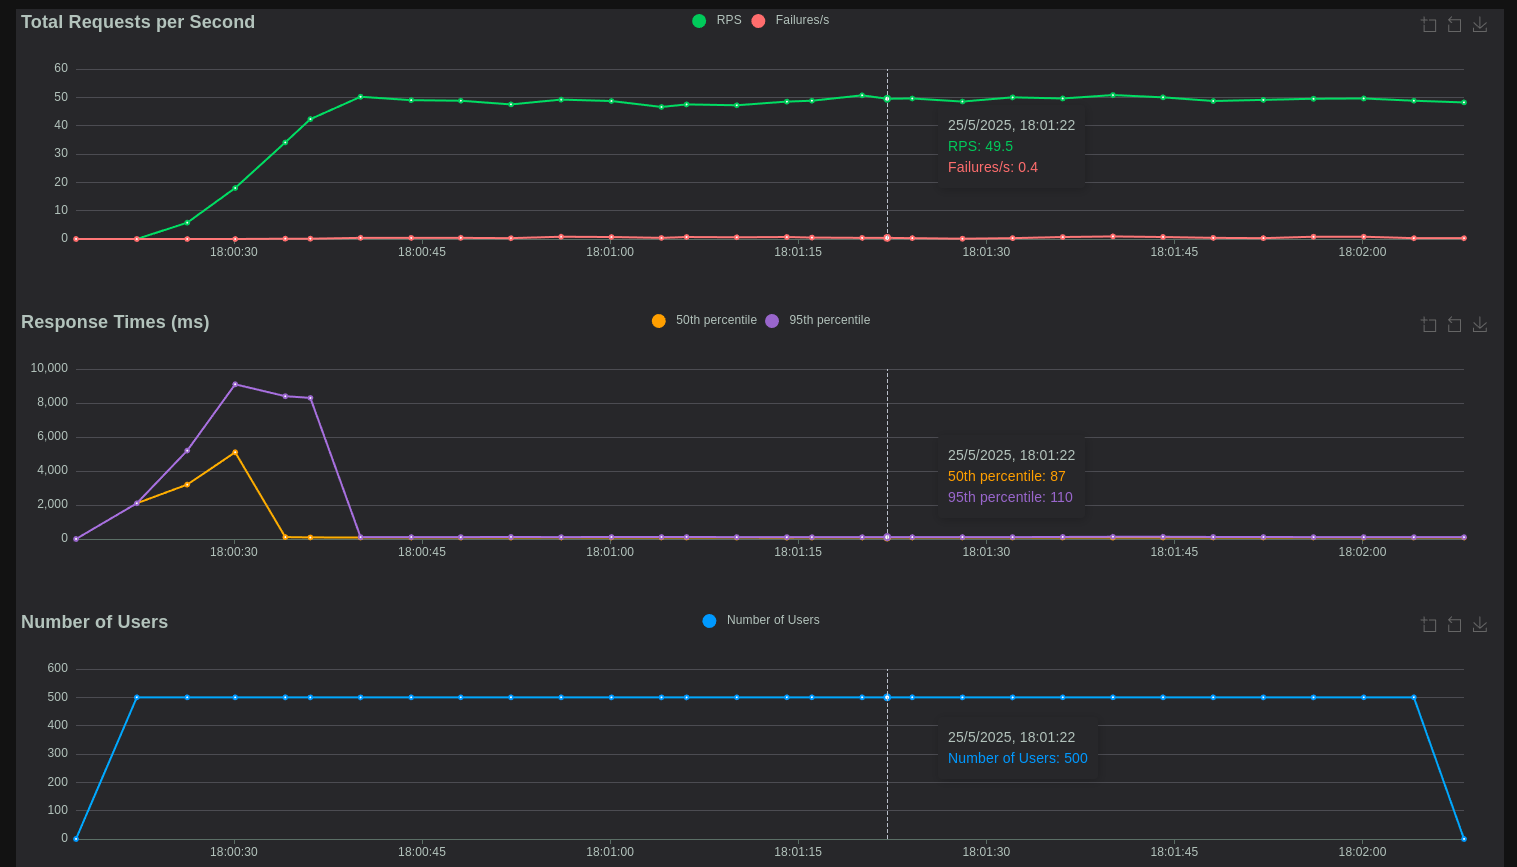
\includegraphics[width=0.9\textwidth]{figures/08_500_1.png}
\caption{Gráfica de la prueba de carga con 500 usuarios concurrentes.}
\label{fig:locust500}
\end{figure}

En esta prueba se observan comporetamientos similares a los de la prueba con 100 usuarios concurrentes, pero con una latencia más alta en general. Esto es esperado, ya que al aumentar el número de usuarios concurrentes, el sistema debe manejar más solicitudes al mismo tiempo, lo que puede aumentar la latencia.
\newline\newline
En la gráfica de ``Response Times (ms)'' se observa un pico de latencia significativa al inicio de la prueba, similar al de la prueba con 100 usuarios concurrentes. En este caso, el percentil 95 alcanzó hasta 9100 ms (9 segundos) y el percentil 50 (mediana) llegó a unos 5100 ms (5 segundos). Posteriormente, los tiempos de respuesta se estabilizaron, lo que es consistente con las estadísticas globales de la prueba, que muestran una mediana de 88 ms y un percentil 95 de 280 ms para el total de la ejecución.
\newline\newline
Además en cuanto a los fallos registrados, una tasa de 48 fallos sobre un total de 4918 solicitudes es también muy baja, representando una tasa de éxito del 99.02\%. Esto indica que el sistema es capaz de manejar una carga moderada de usuarios sin problemas significativos, con tiempos de respuesta aceptables y una tasa de éxito muy alta.
\newline\newline
En resumen, los resultados de la prueba de carga con 500 usuarios concurrentes muestran que el sistema es capaz de manejar una carga moderada de usuarios sin problemas significativos, con tiempos de respuesta aceptables y una tasa de éxito muy alta. Aunque se observan picos de latencia al inicio de la prueba, estos son esperados y no indican un problema grave en el sistema.

\subsubsection{Pruebas de carga con 1000 usuarios concurrentes}

En esta prueba se simularon 1000 usuarios concurrentes realizando solicitudes al sistema durante 2 minutos. Los resultados obtenidos fueron los siguientes:

\begin{table}[H]
\centering
\resizebox{16cm}{!}{
\begin{tabular}{|r|r|r|r|r|r|r|r|r|r|r|}
\hline
\textbf{Req.} & \textbf{Fails} & \textbf{Med(ms)} & \textbf{95\%(ms)} & \textbf{99\%(ms)} & \textbf{Avg(ms)} & \textbf{Min(ms)} & \textbf{Max(ms)} & \textbf{Avg size(Bytes)} & \textbf{RPS} & \textbf{Fails/s} \\
\hline
6672 & 215 & 92 & 2500 & 89000 & 2829.37 & 5 & 135196 & 9404.85 & 50.1 & 0.6 \\
\hline
\end{tabular}
}
\caption{Resultados de la prueba de carga con 1000 usuarios concurrentes.}
\label{tab:locust1000}
\end{table}

\begin{figure}[H]
\centering
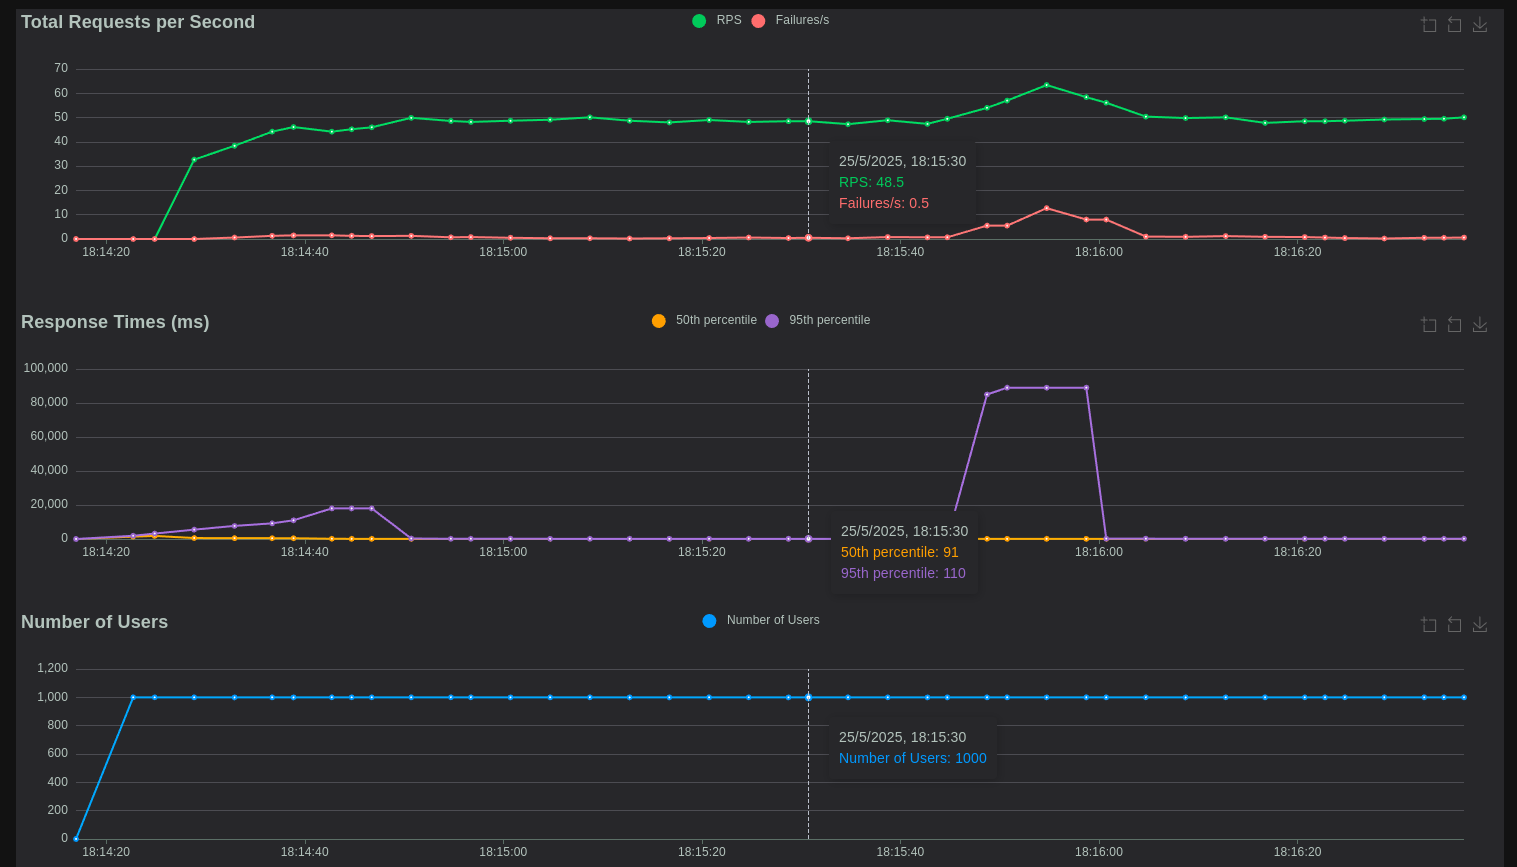
\includegraphics[width=0.9\textwidth]{figures/08_1000_1.png}
\caption{Gráfica de la prueba de carga con 1000 usuarios concurrentes.}
\label{fig:locust1000}
\end{figure}

En este caso se observa un comportamiento similar al de las pruebas anteriores, pero con una latencia aún más alta en general. Esto es esperado, ya que al aumentar el número de usuarios concurrentes, el sistema debe manejar más solicitudes al mismo tiempo, lo que puede aumentar la latencia.
\newline\newline
En la gráfica de ``Response Times (ms)'' se observa un pico de latencia significativa al inicio de la prueba, similar al de las pruebas anteriores. En este caso, el percentil 95 alcanzó hasta 18000 ms (18 segundos) y el percentil 50 (mediana) sin embargo no es tan alto como el de las otras pruebas, llegando a un pico de 140ms al principio. Posteriormente, los tiempos de respuesta se estabilizaron, lo que es consistente con las estadísticas globales de la prueba, que muestran una mediana de 92 ms y un percentil 95 de 2500 ms para el total de la ejecución.
\newline\newline
Además, en cuanto a los fallos registrados, una tasa de 215 fallos sobre un total de 6672 solicitudes es también baja, representando una tasa de éxito del 96.78\%. Aunque esta tasa es inferior a las pruebas anteriores, sigue siendo aceptable y no indica un problema grave en el sistema.
\newline\newline
En esta prueba además se ha observado un comportamiento anómalo alrededor de los 90 segundos de la prueba, donde el percentil 99 alcanzó hasta 89000 ms (89 segundos). Esto indica que hubo un problema puntual en el sistema que afectó a algunas solicitudes, pero no a todas. Este tipo de comportamiento puede deberse a un problema de rendimiento en el servidor o en la base de datos, o a un problema de red.

La ``recuperación'' no se observa en el sentido de que los tiempos de respuesta o fallos vuelvan a niveles óptimos durante esta fase. Más bien, el sistema entra en un estado de alta latencia y fallos continuos bajo esta carga sostenida. La estabilización en el gráfico de tiempos de respuesta a partir de los 80 segundos no es una recuperación positiva, sino una indicación de que el sistema se ha atascado en un estado de rendimiento muy bajo.
\newline
Las causas de esta saturación con 1000 usuarios concurrentes pueden ser:

\begin{itemize}
    \item \textbf{Saturación de recursos del servidor:} Límites de CPU, memoria o procesos en el servicio de aplicación.
    \item \textbf{Cuellos de botella en la base de datos:} Agotamiento del pool de conexiones, contención de bloqueos, o límites de recursos (CPU, RAM, IOPS) en PostgreSQL.
    \item \textbf{Timeouts:} Los tiempos de respuesta excesivos probablemente provocan que las solicitudes excedan los límites de tiempo establecidos, registrándose como fallos.
    \item \textbf{Límites de autoescalado:} Si el autoescalado no es suficientemente rápido o los límites del plan de servicio son insuficientes para 1000 usuarios.
\end{itemize}